\documentclass[14pt,a4paper]{article}
\usepackage[14pt]{extsizes}
\usepackage[left=1.5cm, right=1.5cm, top=1.5cm, bottom=1.5cm]{geometry}
\usepackage[utf8]{inputenc}
\usepackage[T2A]{fontenc}
\usepackage[english, russian]{babel}
\usepackage{amsmath,amsfonts,amssymb,amsthm,mathtools} 
\usepackage{amsfonts}
\usepackage{amssymb}
\usepackage{titleps}
\usepackage{hyperref}
\usepackage{float}
\usepackage{graphicx}
\usepackage{multirow}
\usepackage{hhline}
\usepackage{wrapfig}
\usepackage{tikz}
\usepackage{pgfplots}
\usepackage{xcolor}
\usepackage{subfig}
\usepackage{upgreek}
\usepackage{bm}
\usepackage{longtable}


\newcommand{\w}[1]{\text{#1}}
\newcommand{\und}[1]{\underline{#1}}
\newcommand{\img}[3]{
	\begin{figure}[H]
	\begin{center}
	\includegraphics[scale=#2]{#1}
	\end{center}
	\begin{center}
 	\textit{#3}
	\end{center}
	\end{figure}
}
\newcommand{\aw}[1]{
	\begin{center}
	\textit{#1}
	\end{center}
	\n
}
\newcommand{\be}[1]{
	\begin{center}
	\boxed{#1}
	\end{center}
}
\newcommand{\beb}[1]{
	\begin{equation}
	\boxed{#1}
	\end{equation}
}
\newcommand{\eb}[1]{
	\begin{equation}
	#1
	\end{equation}
}
\newcommand{\n}{\hfill \break}
\newcommand{\x}{\cdot}

\begin{document}
\section*{Работа 4.4.1}	
\section*{Амплитудная дифракционная решётка (гониометр)}
\subsection*{Киркича Андрей, Б01-202, МФТИ}
\n\n
\textbf{Цель работы: }
знакомство с работой и настройкой гониометра, определение спектральных характеристик амплитудной решётки.
	\n\n
	\textbf{В работе используются: }
гониометр, дифракционная решётка, ртутная лампа.
\n\n
В работе исследуются спектр ртутной лампы и дисперсия ртутной решётки, определяются период и спектральные характеристики решётки и оценивается влияние ширины пучка на разрешающаую способность.
\n
\section*{Теоретическая справка}

Основное соотношение приближенной теории дифракционной решётки:

	\begin{equation}
	d\sin \varphi_m = m\lambda.
 	\label{main}
	\end{equation}
 \n
Угловая дисперсия $D$ характеризует угловое расстояние между близкими спектральными линиями:
	\begin{equation}
	D = \frac{d\varphi}{d\lambda} = \frac{m}{d \cos \varphi}=\frac{m}{\sqrt{d^{2}-m^{2} \lambda^{2}}}.
	\end{equation}
\n
Рассмотрим изображения спектра для двух узких спектральных линий с длинами волн $\lambda$ и $\lambda+\delta\lambda$. Для минимального значения $\lambda+\delta\lambda$, которое может быть определено по результатам измерений, вводят важнейшую характеристику спектрального прибора — разрешающую способность:

\begin{equation}
    R=\frac{\lambda}{\delta\lambda}.
\end{equation}


\section*{Экспериментальная установка}

\subsection*{Устройство гониометра}

Гониометр служит для точного измерения углов и находит широкое применение в оптических лабораториях.

\begin{center}
    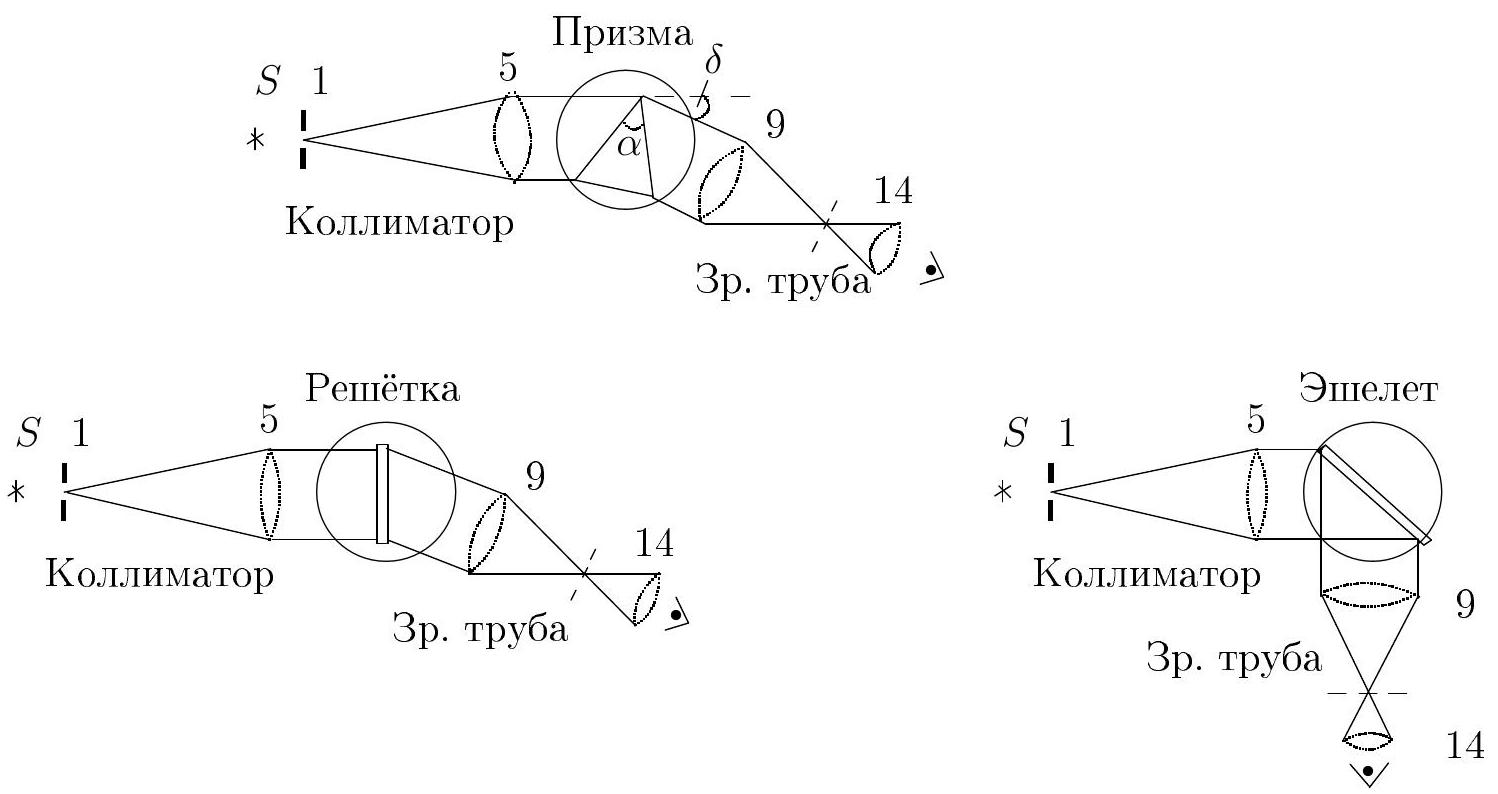
\includegraphics[scale=0.2]{2023_04_02_a48ae02e429ba186bcd7g-2}
\end{center}

\begin{center}
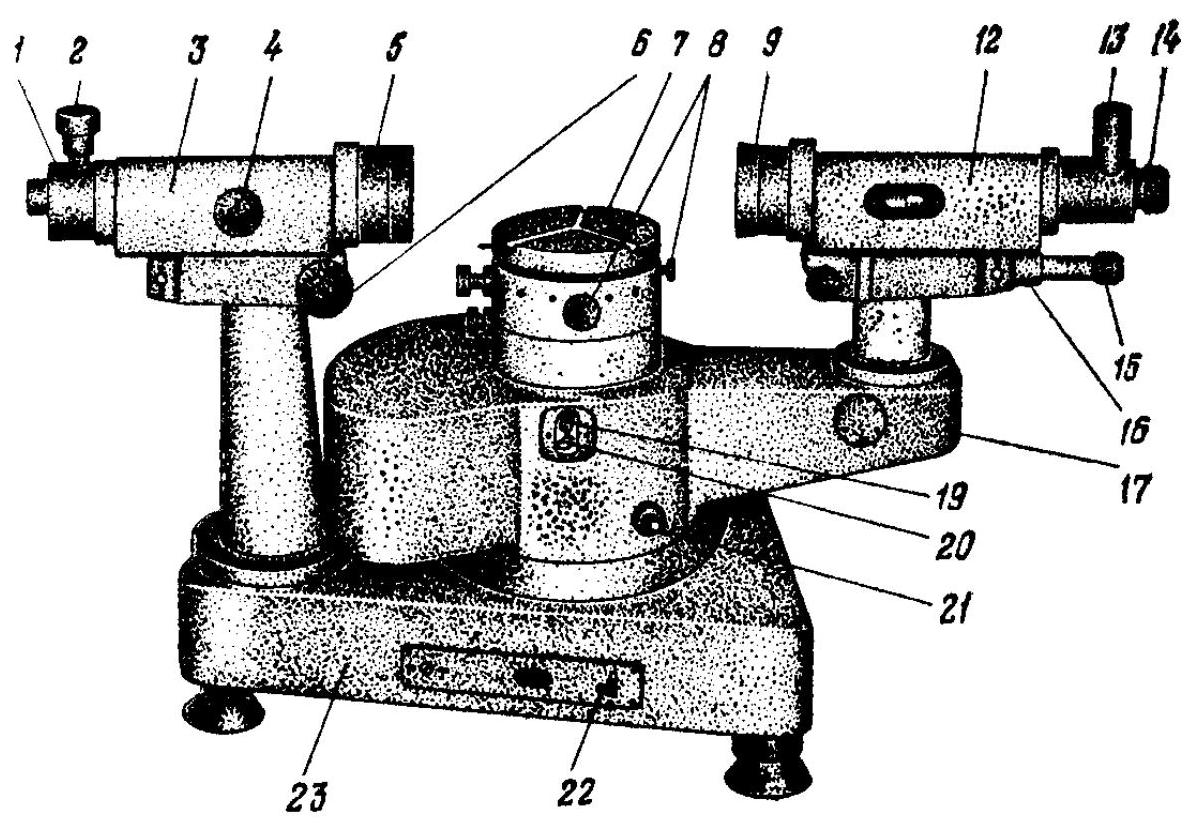
\includegraphics[scale=0.2]{2023_04_02_a48ae02e429ba186bcd7g-2(2)}
\end{center}

\begin{center}
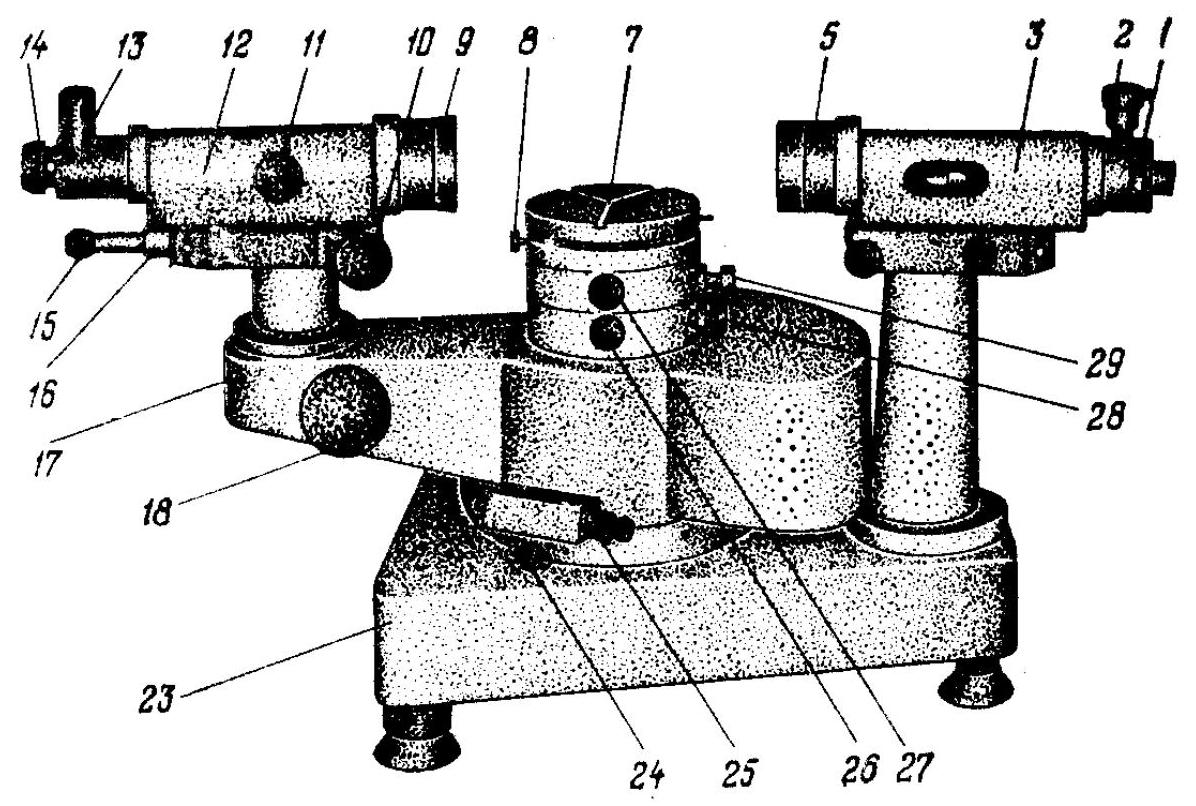
\includegraphics[scale=0.2]{2023_04_02_a48ae02e429ba186bcd7g-2(1)}

Оптическая схема и внешний вид гониометра

\end{center}

\subsection*{Ртутная лампа}

Характеристики спектра ртутной лампы привдены в таблице ниже.

\begin{center}
\begin{tabular}{|c|c|c|c|c|c|c|c|c|}
\hline
№ & $\mathrm{K}_{1}$ & $\mathrm{~K}_{2}$ & 1 & 2 & 3 & 4 & 5 & 6 \\
\hline
$\lambda$ нм. & 690,7 & 623,4 & 579,1 & 577,0 & 546,1 & 491,6 & 435,8 & 404,7 \\
\hline
Цвет & красн. & красн. & желт. & желт. & зелен. & голуб. & синий & фиолет. \\
\hline
Яркость & 4 & 4 & 10 & 8 & 10 & 4 & 4 & 3 \\
\hline
\end{tabular}
\end{center}

\section*{Ход работы}

Сначала были измерены углы для максимумов линий спектра ртутной лампы порядков $\pm 1$. Полученные данные приведены в Таблице \ref{angles}.

\begin{table}[H]
    \centering
    \begin{tabular}{|p{2cm}|p{4cm}|p{4cm}|}
    \hline  \centering{№ линии} & 1 порядок & -1 порядок \\ \hline
$6$   & $11^{\circ} 41^{\prime} 57^{\prime \prime}$  & $11^{\circ} 38^{\prime} 29^{\prime \prime}$  \\ \hline
$5$   & $12^{\circ} 36^{\prime} 34^{\prime \prime}$  & $12^{\circ} 33^{\prime} 37^{\prime \prime}$  \\ \hline
$4$   & $14^{\circ} 15^{\prime} 39^{\prime \prime}$  & $14^{\circ} 11^{\prime} 58^{\prime \prime}$  \\ \hline
$3$   & $15^{\circ} 52^{\prime} 33^{\prime \prime}$  & $15^{\circ} 48^{\prime} 17^{\prime \prime}$  \\ \hline
$2$   & $16^{\circ} 48^{\prime} 04^{\prime \prime}$  & $16^{\circ} 43^{\prime} 18^{\prime \prime}$  \\ \hline
$1$   & $16^{\circ} 51^{\prime} 56^{\prime \prime}$  & $16^{\circ} 47^{\prime} 01^{\prime \prime}$  \\ \hline
$K_2$ & $17^{\circ} 52^{\prime} 08^{\prime \prime}$  & $17^{\circ} 47^{\prime} 11^{\prime \prime}$  \\ \hline
$K_1$ & $18^{\circ} 12^{\prime} 43^{\prime \prime}$  & $18^{\circ} 06^{\prime } 48^{\prime \prime}$  \\ \hline
    \end{tabular}
    \caption{Углы линий спектра ртути}
    \label{angles}
\end{table}
\n
Далее для оценки угловой дисперсии решётки были измерены угловые координаты линий жёлтого дублета для всех видимых порядков спектра, положительных и отрицательных. Данные представлены в таблице \ref{yell}.

\begin{table}[H]
    \centering
    \begin{tabular}{|r|p{4cm}|p{4cm}|}
    \hline $m$ & $\varphi_{1}$ & $\varphi_{2}$ \\ \hline
$-3$  & $59^{\circ} 13^{\prime} 38^{\prime \prime}$  & $59^{\circ} 35^{\prime} 05^{\prime \prime}$  \\ \hline
$-2$  & $35^{\circ} 03^{\prime} 45^{\prime \prime}$  & $35^{\circ} 12^{\prime} 46^{\prime \prime}$  \\ \hline
$-1$  & $16^{\circ} 43^{\prime} 18^{\prime \prime}$  & $16^{\circ} 47^{\prime} 01^{\prime \prime}$  \\ \hline
$1$   & $16^{\circ} 48^{\prime} 04^{\prime \prime}$  & $16^{\circ} 51^{\prime} 56^{\prime \prime}$  \\ \hline
$2$   & $35^{\circ} 24^{\prime} 15^{\prime \prime}$  & $35^{\circ} 33^{\prime} 12^{\prime \prime}$  \\ \hline
$3$   & $60^{\circ} 41^{\prime} 58^{\prime \prime}$  & $61^{\circ} 04^{\prime}  30^{\prime \prime}$  \\ \hline
    \end{tabular}
    \caption{Углы жёлтых линий}
    \label{yell}
\end{table}
\n
Наконец, для оценки разрешающей способности спектрального прибора была измерена угловая ширина одной из линий жёлтого дублета по нулям интенсивности в первом и втором порядках. Угловая ширина составила $\Delta \varphi_1 = 1^{\prime}  30^{\prime \prime}$ и $ \Delta \varphi_2 = 1^{\prime}  53^{\prime \prime}$ соответственно.

\section*{Обработка данных}

По полученным данным был построен график на рис. \ref{angle} зависимости $\sin \varphi_m$ от длины волны. По коэффициенту наклона c использованием формулы \eqref{main} был найден период решётки $d = \frac{1}{k} = 2.04 \pm 0.05$ мкм.

\begin{figure}[H]
    \centering
    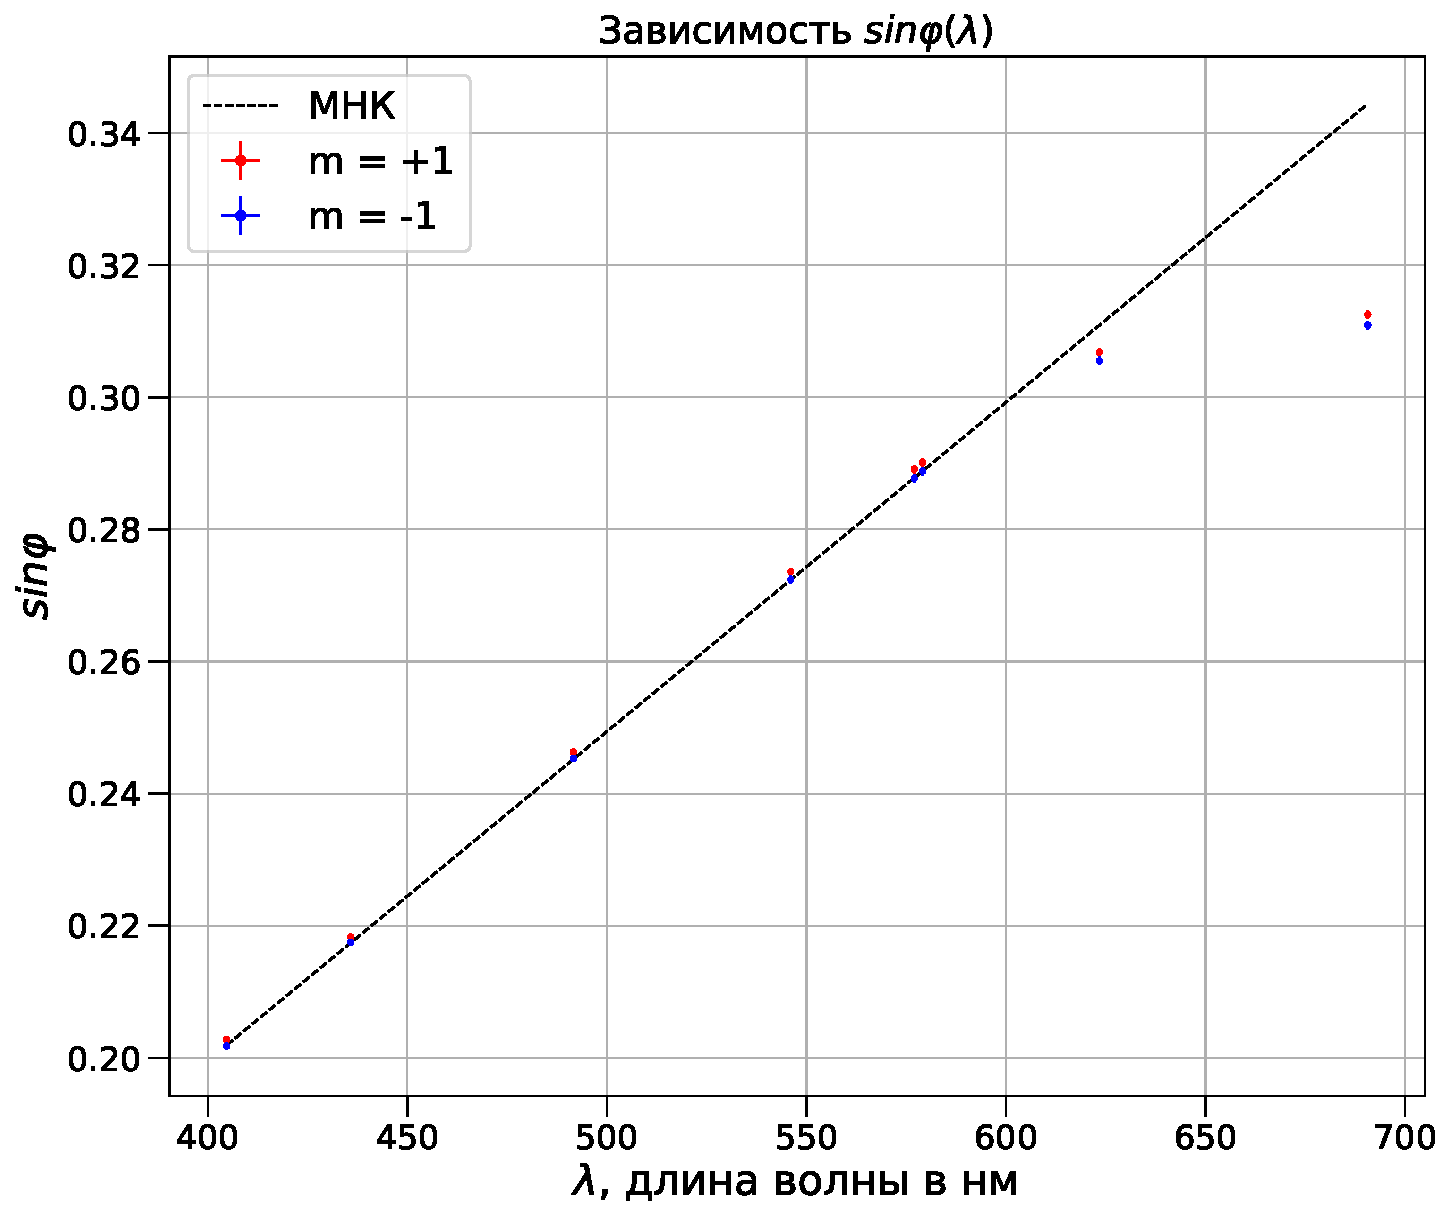
\includegraphics[scale=0.45]{sin.pdf}
    \caption{График зависимости $\sin \varphi$ от длины волны для первых максимумов}
    \label{angle}
\end{figure}
\n
Далее изучим зависимость $D$ от $m$ и сравним результат с формулой 2. Результат наглядно представлен на рисунке \ref{D}.

\begin{figure}[H]
    \centering
    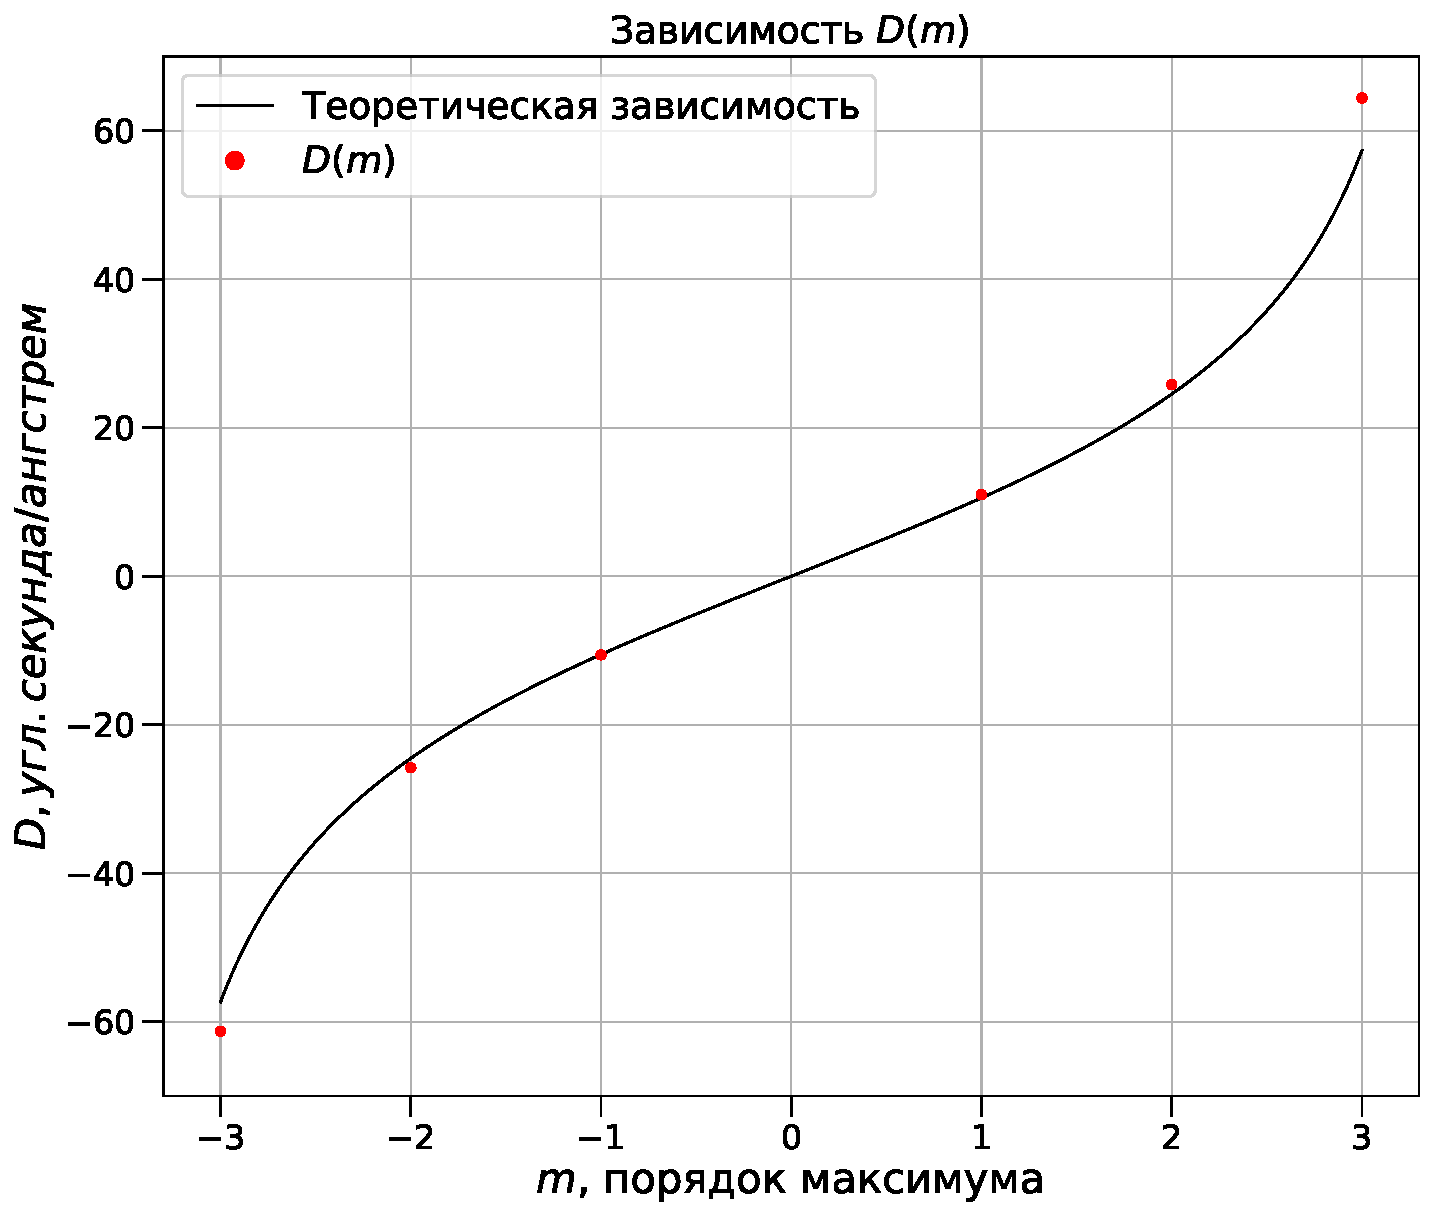
\includegraphics[scale=0.45]{D.pdf}
    \caption{\centering Зависимость угловой дисперсии от порядка}
    \label{D}
\end{figure}
\n
Черная прямая - это теоретическая зависимость, построенная по параметру $d$, ранее определенному. Легко видеть, что теория очень хорошо описывает эксперимент
\n
Определим также разрешающую способность по формуле $\displaystyle R = \frac{\lambda}{\delta \lambda} \approx 680$, число рабочих штрихов решётки $N \approx 680$ и размер освещённой части $l = Nd \approx 1.36$ мм.

\section*{Заключение}

Мы исследовали спектральные линии ртути, определили шаг решётки, её угловую дисперсию, а также её разрешающую способность. Полученные результаты близки к теоретическим предсказаниям.

\end{document}
